\chapter{V2V Main Structure}
In this chapter, a sneak peek inside the vehicle unit of the connected vehicles will be shown as well as the server unit.\newline
In order to see a complete picture of the project, this chapter seeks to provide a brief overview of the ICs and modules used, their functions, and how they are connected to one another as well as how the cars are connected to one another. It will also provide summary of steps that are followed to complete the project.\newline

\section{Project Design}
In this section, the diagram of the project and components that were used and their purposes are viewed.

\subsection{Diagram}
Figure \ref{fig:block-diagram} shows the main construction, and how the vehicles communicate together using a server. It also shows the name for each component and the connection of the components inside each vehicle unit. 
\begin{figure}[h]
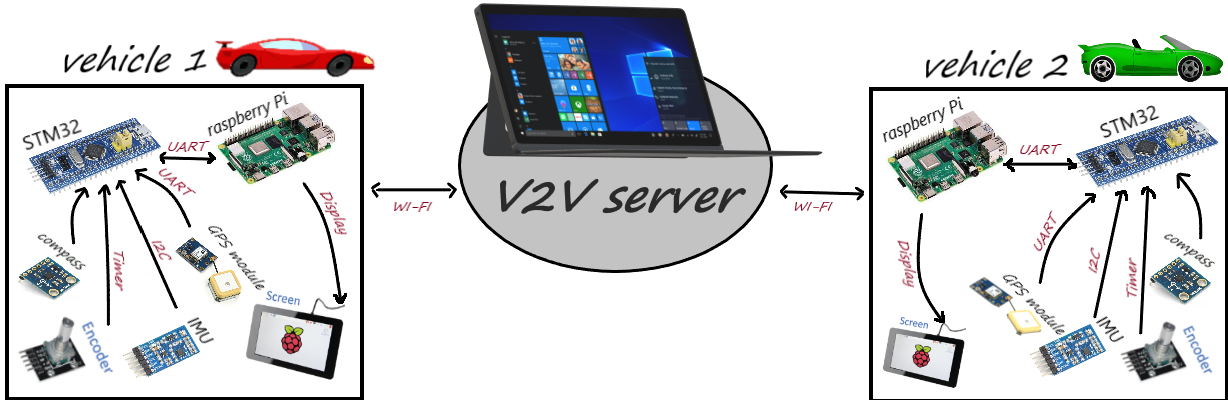
\includegraphics[width=\textwidth]{figure/2_1.png}
\caption{Block diagram of the project}
\label{fig:block-diagram}
\centering
\end{figure}

\subsection{Vehicle Unit}

The employed micro-controller, the STM32F103C8, handles data from the car connected to it as well as data from nearby cars. As a result, it must collect and analyze incoming data. In order to achieve this, as shown figure \ref{fig:vehicle-unit}, the STM is connected to:
\begin{itemize}
    \item \textbf{STM32F103C8: } It's the micro-controller which contains the analysis of the project. It is the processor of the project.
    \item \textbf{Raspberry Pi: }The Raspberry Pi serves as a link between a car and its neighboring cars. It communicates with STM using UART serial communication protocol and with the server via Wi-Fi. It also helps the user by providing a Graphical User Interface (GUI) system.
    \item \textbf{An inertial measurement unit (IMU): } The chosen IMU is GY-521 MPU6050 since it is based on Micro Electro-Mechanical Systems (MEMS) technology  which allows lower costs and low power requirements while ensuring performance. \newline
    The MPU-6050 sensor module measures acceleration, orientation, angular rates of the vehicle and reports it to the STM32 through an Inter-Integrated-Circuit (I2C) serial communication bus.
    \item \textbf{Inferred Rotary (IR) encoder: } The encoder which provides data on the rotating shaft's rotation angle and rotational speed (RPM).
    \item \textbf{Global Positioning System (GPS) module: }The GPS module, which is coupled to the STM32 through Universal asynchronous receiver-transmitter (UART) serial communication protocol, provides information about the car's location. \newline
    Note: Because of the weakness of GPS connection, it is replaced by Bluetooth module which receives the GPS data from mobile by Bluetooth and sends it to STM using UART.
    \item \textbf{compass module: } Compass provides STM with the angle between the vehicle and north direction.
    \item \textbf{Screen: } The screen is used to display the data for the user.
\end{itemize}

\begin{figure}
    \centering
    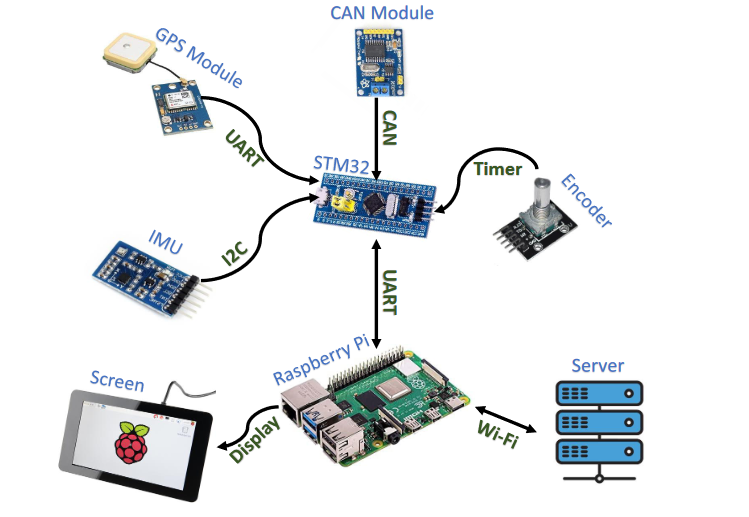
\includegraphics[width = \textwidth]{figure/2_1_1.PNG}
    
    \caption{Diagram for V2V vehicle unit}
    \label{fig:vehicle-unit}
\end{figure}

\newpage
\subsection{Server Unit}
The server used in that project is actually a laptop. All Raspberry Pi boards inside the system of V2V must be connected through Wi-Fi to the server in order to send and receive data in the form of JSON files anytime. \newline
 The server receives data from any connected vehicle and sends this data to all other connected cars. After receiving a JSON file, Raspberry Pi converts it into a string to be sent to the STM, by the same time, STM extracts data from the mentioned sensors and modules, and then it analyzes both data from its vehicle and from the neighboring vehicle and gives a warning message if an action must be taken to avoid a collision.\newline
 
 \section{Project Steps}
 This section will show an overview for the project steps that are followed, the details for each step will be discussed in separate chapters. \newline
 
 To build the vehicle unit, it is needed to follow these steps:
 \begin{enumerate}
     \item Drivers’ initialization: first of all, all drivers for STM protocols and peripherals are initialized, this step must be done before project implementation. The details will be discussed in chapter 4.
     \item Sensors and modules interfacing: After initialization of all needed drivers, sensors and modules are implemented and interfaced with STM to be ready to send and receive data. Details for each module and sensor interfacing are discussed in chapter 5.
     \item Data Analysis: After interfacing with sensors which provide STM with vehicle data, this data is analyzed for detecting any future accidents may be happened. Details for analysis and algorithms are discussed in chapter 6.
 \end{enumerate}
 
 
 The server unit is responsible for exchanging information between vehicles, the implementation steps are as follows:
 
 \begin{enumerate}
     \item Simplex System: a simple program is written to send the data in only one way.
     \item Duplex System: After ensuring that the simplex code works correctly, it is improved to be able to send and receive information.
     \item Multiple files: The program needs to be able to handle sending and receiving multiple files.
     \item Multiple clients: The Program has to handle more than one client.
     \item GUI: The server provided a simple GUI for administration.
\end{enumerate}
 After these steps, the server works properly as data is sent from one client to the server in JavaScript Object Notation (JSON) format, then the server sends it to other clients, these clients receive the data in JSON format, then it converts it into string to be sent to STM. Inner workings of the server will be discussed in chapter 7. \newline
 Now, both V2V unit and server unit are implemented separately, the next step would be to have them communicate with each other.
 
 Hardware implementation is discussed in chapter 8.
 
 